\comment{Suggestion: past tense}\\

\subsection{Gradient Descent analysis}
    \begin{figure*}
        \begin{subfigure}{.5\textwidth}
            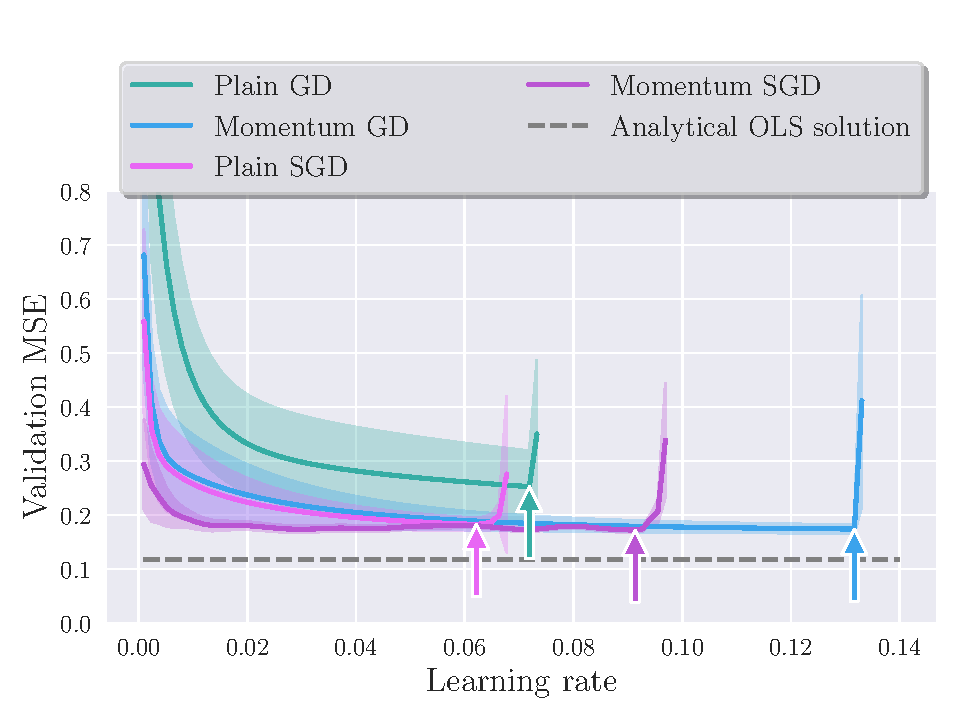
\includegraphics[width=\linewidth]{learning_rates_PGD_MGD_PSGD_MSGD.pdf}
            \caption{Best MSEs, learning rates: (0.2589, 0.0681), (0.1684, 0.126), (0.1738, 0.0384), (0.1709, 0.00874)}
            \label[fig]{res:fig:lrate1}
        \end{subfigure}
        \hfill
        \begin{subfigure}{.5\textwidth}
            \centering
            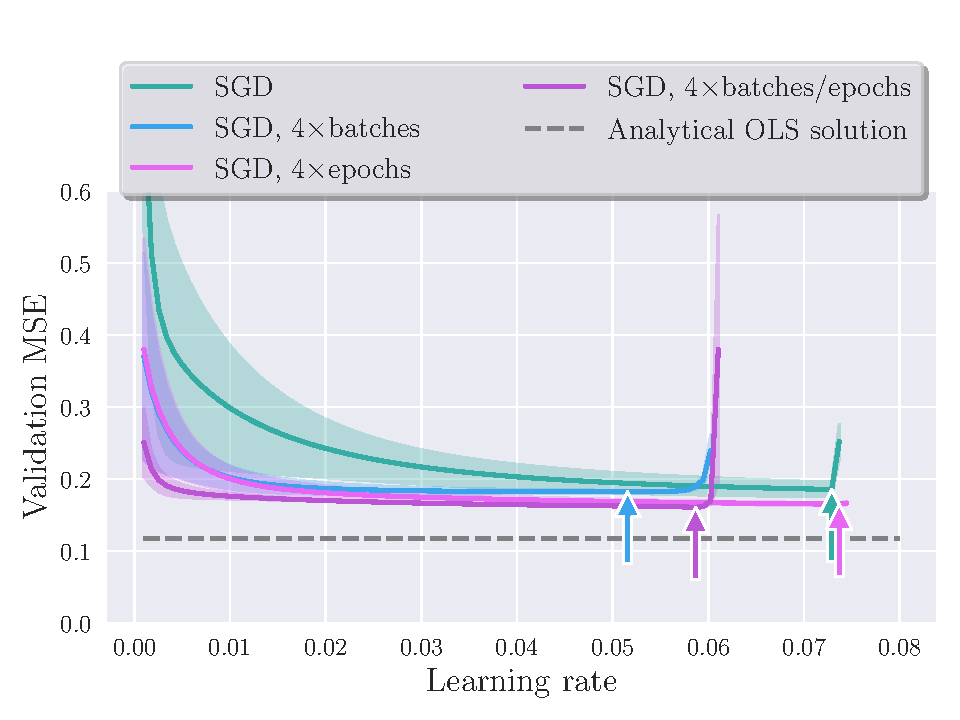
\includegraphics[width=\linewidth]{learning_rates_SGD_batches_epochs.pdf}
            \caption{Best MSEs, learning rates: (0.1738, 0.0382), (0.1692, 0.167), (0.1647, 0.0329), (0.1634, 0.00394)}
            \label[fig]{res:fig:lrate2}
        \end{subfigure}
        \hfill
        \begin{subfigure}{.5\textwidth}
            \centering
            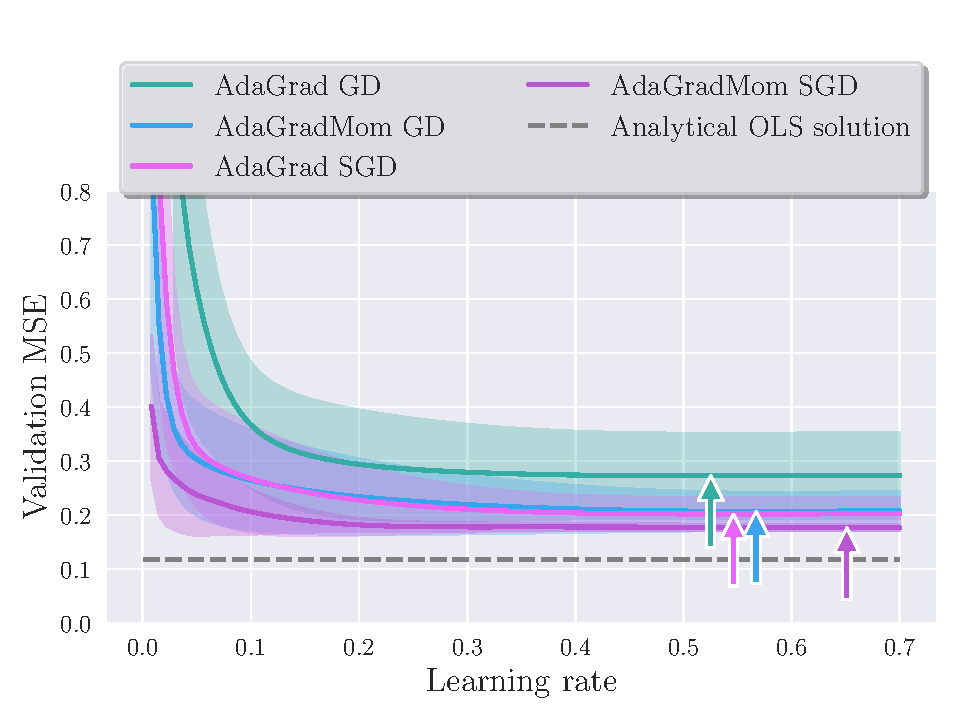
\includegraphics[width=\linewidth]{learning_rates_adagrad}
            \caption{Best MSEs, learning rates: (0.2739, 0.498), (0.2058, 0.564), (0.1764, 0.522), (0.1709, 0.187)}
            \label[fig]{res:fig:lrate3}
        \end{subfigure}
        \caption{Plots of the validation MSE of the parameters found from optimising the OLS cost function on Franke function data with $n=600$ data points. For the momentum methods we used $\gamma=0.8$. The stochastic methods used 16 batches and 100 epochs, while the standard GD did 100 iterations unless specified otherwise.}
        \label[fig]{res:fig:lrates}
    \end{figure*}